\documentclass[10pt,a4paper]{article}
\usepackage{booktabs}
\usepackage[utf8]{inputenc}
\usepackage[T1]{fontenc}
\usepackage[spanish, es-tabla]{babel}
\usepackage{amsmath, amsfonts, amssymb, amsthm}
\usepackage{graphicx}
\usepackage[left=2.54cm, right=2.54cm, top=2.54cm, bottom=2.54cm]{geometry}
\usepackage{tikz}
\usepackage{soul}
\usepackage{listings}
\usepackage[most]{tcolorbox}
\usepackage{float}
\tcbset{shield externalize}
\usetikzlibrary{arrows.meta, positioning, automata}
\usetikzlibrary{babel}
\usepackage{hyperref}

%--------------------------------------------------------------------------------

% Bloque de Ejercicio
\newtcbtheorem[number within=section]{ejercicio}{Ejercicio}{
    enhanced,
    sharp corners,
    boxrule=0pt,
    leftrule=5pt,
    colframe=gray!30!black,
    colback=gray!5!white,
    coltitle=white,
    fonttitle=\bfseries,
    separator sign={.\ },
    before skip=10pt,
    after skip=10pt
}{ej}

% Bloque de Teoremas
\newtcbtheorem[number within=section]{mytheo}{Teorema}{
    enhanced,
    sharp corners,
    boxrule=0pt,
    leftrule=5pt,
    colframe=blue!40!black,
    colback=blue!5!white,
    coltitle=white,
    fonttitle=\bfseries,
    separator sign={.\ },
    before skip=10pt,
    after skip=10pt
}{th}

 % Bloque de Alerta
\newtcolorbox{alerta}[1]{
    enhanced,
    sharp corners,
    boxrule=0pt,
    leftrule=5pt,
    colframe=red!40!black,
    colback=red!5!white,
    coltitle=white,
    fonttitle=\bfseries,
    title=#1,
    before skip=10pt,
    after skip=10pt
}

% Bloque de Notas
\newtcolorbox{nota}[1]{
    enhanced,
    sharp corners,
    boxrule=0pt,
    leftrule=5pt,
    colframe=orange!40!black,
    colback=yellow!5!white,
    coltitle=white,
    fonttitle=\bfseries,
    title=#1,
    before skip=10pt,
    after skip=10pt
}

% ---------------------------------------------------------------------------------------------
\begin{document}

\begin{titlepage}
    \centering
    {\huge \textbf{Universidad Nacional Autónoma de México}}\\[0.3cm]
    \rule{\linewidth}{2mm}\\[0.3cm]
    {\large \textbf{Facultad de Estudios Superiores Acatlán}}\\[1cm]
    

    
\includegraphics[width=6cm]{../../Archivos/Imagenes_Logos/acatlan.png}\\[1cm]
    
    {\Large \textbf{Matemáticas Aplicadas y Computación}}\\[1cm]
    {\huge \textbf{Optimización 2}}\\[0.5cm]
    \rule{\linewidth}{0.3mm}\\[0.3cm]
    {\Large \textit{Redes de Optimización Flujo Máximo y Corte Mínimo}}\\[0.3cm]
    \rule{\linewidth}{0.3mm}\\[0.3cm]
    
    \vfill
    
    \rule{\linewidth}{0.5mm}\\[0.3cm]
    {\Large \textit{Ricardo López Ramírez}}\\
    \rule{\linewidth}{0.5mm}\\[0.8cm]
    
 \small
    Actualización: \today \hfill Página: \thepage
\end{titlepage}

% ÍNDICE 
\pagenumbering{roman}
\tableofcontents
\cleardoublepage
\pagenumbering{arabic}
\setcounter{page}{1}

% CONTENIDO 
\section{Flujo Máximo y Corte Mínimo}

\begin{ejercicio}{Encontrar el corte de capacidad mínima}{a}
Suponer las capacidades dadas en la red. Encontrar el corte de capacidad mínima y verificar el resultado calculando el flujo máximo.
\end{ejercicio}

\subsection{Construcción y Representación de la Red}

Modelo de red dirigida con un nodo fuente ($S$) y un 
nodo sumidero ($t$). Las aristas poseen una capacidad 
máxima $c_{ij}$ que restringe la cantidad de flujo que 
puede circular entre el nodo $i$ y el nodo $j$.

\begin{center}
\begin{tikzpicture}[
    every node/.style={circle, draw, minimum size=0.9cm, font=\sffamily\small\bfseries},
    source_sink/.style={fill=gray!80!black, text=white},
    regular_node/.style={fill=red!40},
    edge/.style={->, >=stealth, thick, color=gray!80!black}
]

% Nodos
\node[source_sink] (S) at (0, 0) {S};
\node[regular_node] (1) at (3, 2.5) {1};
\node[regular_node] (2) at (3, 0) {2};
\node[regular_node] (3) at (3, -2.5) {3};
\node[regular_node] (4) at (6, 0) {4};
\node[regular_node] (5) at (9, 2.5) {5};
\node[regular_node] (6) at (9, 0) {6};
\node[regular_node] (7) at (9, -2.5) {7};
\node[source_sink] (t) at (12, 0) {t};

% Aristas y capacidades
\draw[edge] (S) -- node[above left, draw=none, fill=none] {30} (1);
\draw[edge] (S) -- node[above, draw=none, fill=none] {10} (2);
\draw[edge] (S) -- node[below left, draw=none, fill=none] {15} (3);

\draw[edge] (1) -- node[above, draw=none, fill=none] {1} (5);
\draw[edge] (1) -- node[above right, draw=none, fill=none, pos=0.3] {15} (4);
\draw[edge] (1) -- node[left, draw=none, fill=none] {2} (2);

\draw[edge] (2) -- node[above, draw=none, fill=none] {7} (4);
\draw[edge] (2) -- node[left, draw=none, fill=none] {5} (3);

\draw[edge] (3) -- node[above left, draw=none, fill=none, pos=0.3] {4} (4);
\draw[edge] (3) -- node[above, draw=none, fill=none] {5} (7);

\draw[edge] (4) -- node[above left, draw=none, fill=none, pos=0.3] {10} (5);
\draw[edge] (4) -- node[above, draw=none, fill=none] {30} (6);
\draw[edge] (4) -- node[below left, draw=none, fill=none, pos=0.3] {10} (7);

\draw[edge] (5) -- node[above right, draw=none, fill=none] {15} (t);
\draw[edge] (6) -- node[above, draw=none, fill=none] {20} (t);
\draw[edge] (7) -- node[below right, draw=none, fill=none] {40} (t);

\end{tikzpicture}
\end{center}

\subsection{Aplicación del Algoritmo de Flujo Máximo (Ford-Fulkerson)}

Para encontrar el corte mínimo.
Llevar la red a su estado de flujo máximo. 
Método de las trayectorias de aumento, 
enviando flujo a través de caminos factibles desde $S$
 hasta $t$ hasta saturar los cuellos de botella.

\begin{table}[h!]
\centering
\begin{tabular}{|c|l|c|c|}
\hline
\textbf{Iteración} & \textbf{Ruta de Aumento (Camino)} & \textbf{Capacidad Mínima ($\Delta f$)} & \textbf{Flujo Acumulado} \\ \hline
1 & $S \to 1 \to 4 \to 6 \to t$ & $\min(30, 15, 30, 20) = 15$ & 15 \\ \hline
2 & $S \to 1 \to 5 \to t$       & $\min(15, 1, 15) = 1$       & 16 \\ \hline
3 & $S \to 2 \to 4 \to 6 \to t$ & $\min(10, 7, 15, 5) = 5$    & 21 \\ \hline
4 & $S \to 2 \to 4 \to 7 \to t$ & $\min(5, 2, 10, 40) = 2$    & 23 \\ \hline
5 & $S \to 3 \to 4 \to 7 \to t$ & $\min(15, 4, 8, 38) = 4$    & 27 \\ \hline
6 & $S \to 3 \to 7 \to t$       & $\min(11, 5, 34) = 5$       & 32 \\ \hline
\end{tabular}
\caption{Iteraciones del Algoritmo de Ford-Fulkerson.}
\end{table}

\begin{nota}{Análisis de Rutas}
Desde $S$ aún podríamos enviar flujo hacia los 
nodos 1, 2 y 3 (tienen capacidades residuales de 14, 3 y 6 respectivamente). 
todos los arcos de salida hacia los nodos 4, 5 y 7 
($1 \to 4$, $1 \to 5$, $2 \to 4$, $3 \to 4$, $3 \to 7$) 
están \textbf{saturados}. 
No hay ningún camino residual activo que permita llegar hasta $t$. El \textbf{Flujo Máximo} del sistema es \textbf{32}.
\end{nota}

\newpage

\subsection{Corte Mínimo}

Dividimos los nodos del grafo en dos conjuntos mutuamente excluyentes 
$A$ y $B$, basándonos en la red residual final:

\begin{itemize}
    \item \textbf{Conjunto $A$ :} Incluye a $S$ y a todos los nodos a los que se puede llegar a través de arcos que aún no están saturados. $A = \{S, 1, 2, 3\}$.
    \item \textbf{Conjunto $B$ :} El resto de los nodos, incluyendo el sumidero. $B = \{4, 5, 6, 7, t\}$.
\end{itemize}

El corte se define por los arcos que nacen en el conjunto $A$ y terminan en el conjunto $B$. Estos arcos son los verdaderos "cuellos de botella" estructurales de la red:
$ Corte(A,B) = \{ (1,5), (1,4), (2,4), (3,4), (3,7) \} $

Calculamos la capacidad total del corte sumando las capacidades originales de estos arcos:
$ C(A,B) = c(1,5) + c(1,4) + c(2,4) + c(3,4) + c(3,7) $
$ C(A,B) = 1 + 15 + 7 + 4 + 5 = \mathbf{32} $

\subsection{Resultados}

\begin{mytheo}{Teorema de Flujo Máximo y Corte Mínimo}{maxflow_mincut}
En cualquier red de transporte, el valor del flujo máximo desde el nodo fuente hasta el nodo sumidero es estrictamente igual a la capacidad del corte mínimo que separa a ambos nodos.
$ f_{\max} = C_{\min}(A,B) $
\end{mytheo}

Al comparar nuestros resultados empíricos:
\begin{itemize}
    \item Flujo Máximo Obtenido = \textbf{32 unidades}
    \item Capacidad del Corte Mínimo = \textbf{32 unidades}
\end{itemize}

\begin{alerta}{Conclusión}
El sistema está limitado estructuralmente por la capacidad de paso desde los nodos 
$\{1,2,3\}$ hacia los nodos posteriores de la red, y es imposible enviar más de 32 unidades bajo 
las restricciones actuales.
\end{alerta}

\newpage

\section{Aplicación del Método de Flujo Mínimo}

\begin{ejercicio}{Red de Ductos de Agua (Veracruz)}{b}
Se requiere saber cuál es la cantidad mínima de agua 
que debe circular en la red desde la fuente
 ($S$) hasta el sumidero ($t$) para cubrir los 
 \textbf{requerimientos mínimos} $l_{ij}$ de cada 
 ducto, basándonos en el análisis del video 
 proporcionado.
\end{ejercicio}

\subsection{Representación de la Red}

Red representativa con requerimientos mínimos
$l_{ij}$.

\begin{center}
\begin{tikzpicture}[
    every node/.style={circle, draw, minimum size=0.8cm, font=\sffamily\small\bfseries},
    source_sink/.style={fill=gray!80!black, text=white},
    regular_node/.style={fill=cyan!40},
    edge/.style={->, >=stealth, thick, color=gray!80!black}
]

% Nodos
\node[source_sink] (S) at (0, 0) {S};
\node[regular_node] (1) at (3, 3) {1};
\node[regular_node] (2) at (3, 0) {2};
\node[regular_node] (3) at (3, -3) {3};
\node[regular_node] (4) at (6, 2) {4};
\node[regular_node] (5) at (6, 0) {5};
\node[regular_node] (6) at (6, -2) {6};
\node[source_sink] (t) at (9, 0) {t};

% Arcos y Requerimientos (l_ij)
\draw[edge] (S) -- node[above left, draw=none, fill=none] {11} (1);
\draw[edge] (S) -- node[above, draw=none, fill=none] {15} (2);
\draw[edge] (S) -- node[below left, draw=none, fill=none] {9} (3);

\draw[edge] (1) -- node[above right, draw=none, fill=none] {4} (4);
\draw[edge] (1) -- node[left, draw=none, fill=none, pos=0.7] {5} (5);

\draw[edge] (2) -- node[below left, draw=none, fill=none, pos=0.3] {8} (4);
\draw[edge] (2) -- node[above, draw=none, fill=none] {7} (5);
\draw[edge] (2) -- node[above left, draw=none, fill=none, pos=0.3] {5} (6);

\draw[edge] (3) -- node[left, draw=none, fill=none, pos=0.7] {2} (5);
\draw[edge] (3) -- node[below right, draw=none, fill=none] {4} (6);

\draw[edge] (4) -- node[above right, draw=none, fill=none] {9} (t);
\draw[edge] (5) -- node[above, draw=none, fill=none] {5} (t);
\draw[edge] (6) -- node[below right, draw=none, fill=none] {14} (t);
\draw[edge] (6) -- node[left, draw=none, fill=none] {3} (5);

\end{tikzpicture}
\end{center}

\subsection{Método de Flujo Mínimo}


\textbf{Asignar un flujo inicial ($V_1$) que supere los requerimientos.} \\
Asignamos un flujo arbitrario pero suficiente ($f_{ij} \ge l_{ij}$) manteniendo el equilibrio de los nodos.
\begin{itemize}
    \item Flujo enviado desde $S$: $f(S,1)=20, f(S,2)=30, f(S,3)=20$. \textbf{Flujo Total $V_1 = 70$}.
\end{itemize}

\textbf{Paso 2: Crear la Red Residual con Capacidades Modificadas ($u'_{ij} = f_{ij} - l_{ij}$).}


\begin{table}[h!]
\centering
\begin{tabular}{ccccc}
\toprule
\textbf{Arco} & \textbf{Requerimiento ($l_{ij}$)} & \textbf{Flujo Pasado ($f_{ij}$)} & \textbf{Nueva Capacidad ($u'_{ij}$)} \\
\midrule
(S,1) & 11 & 20 & \textbf{9} \\
(S,2) & 15 & 30 & \textbf{15} \\
(S,3) & 9  & 20 & \textbf{11} \\
(1,4) & 4  & 10 & \textbf{6} \\
(1,5) & 5  & 10 & \textbf{5} \\
(2,4) & 8  & 10 & \textbf{2} \\
(2,5) & 7  & 10 & \textbf{3} \\
(2,6) & 5  & 10 & \textbf{5} \\
(3,5) & 2  & 10 & \textbf{8} \\
(3,6) & 4  & 10 & \textbf{6} \\
(4,t) & 9  & 20 & \textbf{11} \\
(5,t) & 5  & 35 & \textbf{30} \\
(6,5) & 3  & 5  & \textbf{2} \\
(6,t) & 14 & 15 & \textbf{1} \\
\bottomrule
\end{tabular}
\end{table}

\textbf{Aplicar Ford-Fulkerson para hallar el Flujo Máximo ($V_2$) en la red residual.}

\newpage

Buscamos devolver la mayor cantidad de flujo "sobrante" posible.

\begin{itemize}
    \item Ruta 1: $S \to 1 \to 4 \to t$ ($\min(9,6,11) = \mathbf{6}$)
    \item Ruta 2: $S \to 1 \to 5 \to t$ ($\min(3,5,30) = \mathbf{3}$)
    \item Ruta 3: $S \to 2 \to 4 \to t$ ($\min(15,2,5) = \mathbf{2}$)
    \item Ruta 4: $S \to 2 \to 5 \to t$ ($\min(13,3,27) = \mathbf{3}$)
    \item Ruta 5: $S \to 2 \to 6 \to t$ ($\min(10,5,1) = \mathbf{1}$)
    \item Ruta 6: $S \to 2 \to 6 \to 5 \to t$ ($\min(9,4,2,24) = \mathbf{2}$)
    \item Ruta 7: $S \to 3 \to 5 \to t$ ($\min(11,8,22) = \mathbf{8}$)
\end{itemize}
\textbf{Flujo Máximo de retorno ($V_2$):} $6 + 3 + 2 + 3 + 1 + 2 + 8 = \mathbf{25}$.

\textbf{Calcular el Flujo Mínimo.}
\begin{equation*}
    V_{\min} = V_1 - V_2 = 70 - 25 = \mathbf{45}
\end{equation*}

\subsection{Corte Mínimo}

En la red residual (Paso 3), el algoritmo se detiene 
porque ya no existen caminos con capacidad disponible 
hacia $t$. El conjunto de nodos alcanzables desde $S$ 
en la red residual final y los no alcanzables definen 
el \textbf{Corte de Capacidad Mínima}.
Este corte actúa como la \textbf{barrera de contención}; indica físicamente por qué no podemos restar más de 25 unidades de flujo. De hacerlo, violaríamos el requerimiento de al menos un ducto de la red real.

\subsection{ Capacidades y Requerimientos}

problemas donde conviven requerimientos ($l_{ij}$) y 
capacidades ($u_{ij}$),
 $l_{ij} \le f_{ij} \le u_{ij}$, 
 a teoría de Programación Lineal se adapta:

\begin{nota}{Soluciones en Redes de Flujo}
\begin{itemize}
    \item \textbf{Solución Óptima y Múltiple:} Son los escenarios normales.Puedes haber elegido rutas iniciales diferentes, pero ambos llegaremos indefectiblemente a $V_{\min} = 45$.
    \item \textbf{Solución No Acotada:} \textit{No existe.} Como la red tiene capacidades máximas (o requerimientos fijos), el flujo no puede crecer o decrecer infinitamente.
    \item \textbf{Solución No Factible:} Solo se daría si la suma de capacidades de entrada a un nodo fuera estrictamente menor que su requerimiento de salida, lo cual implicaría un error de diseño estructural.
\end{itemize}
\end{nota}

\subsection{Resultados}

Verificamos el balance del Nodo 5 con los flujos finales reales ($f_{final} = f_{ij} - v_{2,ij}$):
\begin{itemize}
    \item Entradas al Nodo 5: $(10-3) + (10-3) + (10-8) + (5-2) = 7 + 7 + 2 + 3 = \mathbf{19}$.
    \item Salidas del Nodo 5: $(35-16) = \mathbf{19}$.
\end{itemize}

\begin{alerta}{Conclusión}
El nodo 5, al igual que todos los nodos de transbordo de la red, mantiene el equilibrio perfecto (Entrada = Salida = 19). Además, el flujo de salida 19 es mayor a su requerimiento $l_{5t} = 5$. El cálculo es matemáticamente robusto: la cantidad mínima para operar la red es de \textbf{45 unidades}.
\end{alerta}



$(c)$ Llenar tu flor de conocimiento tomando el apunte correspondiente, y realizar el
siguiente enunciado usando flujo mínimo:
Suponer los siguientes requerimientos, aplicar el método de flujos mínimos: 

Como se observa en la Figura \autoref{fig:Pag54} 

Como se observa en la Figura \autoref{fig:Pag55}

Como se observa en la Figura \autoref{fig:Pag56}

\newpage

\section{Flujo Máximo}

\begin{ejercicio}{Red con Requerimientos, Capacidades y Nodos Múltiples}{d,e}
Suponer la red con formato ($l_{ij}, u_{ij}$) (requerimiento, capacidad), 
con capacidades en los nodos ($C(6)=13$) y donde $S$ y $2$ son nodos iniciales, $t$ y $6$ son nodos terminales. Encontrar el flujo máximo.
\end{ejercicio}

\subsection{ Red Ficticia}

Aplicando la teoría desarrollada, reconstruimos la red:
\begin{enumerate}
    \item Creamos un nodo súper-origen $\mathbf{S^*}$ conectado a los nodos iniciales $S$ y $2$ con capacidad $\infty$.
    \item Creamos un nodo súper-sumidero $\mathbf{t^*}$ conectado a los nodos terminales $t$ y $6$ con capacidad $\infty$.
    \item Dividimos el nodo $6$ (cuya capacidad interna es $C(6)=13$) en dos sub-nodos $\mathbf{6'}$ y $\mathbf{6''}$, unidos por un arco dirigido $(6', 6'')$ con capacidad $(0, 13)$. Los arcos de entrada llegan a $6'$, y los de salida nacen en $6''$.
\end{enumerate}

\subsection{Factibilidad}

Ford-Fulkerson, encontrar un flujo factible inicial que satisfaga 
\textbf{todas} las restricciones $l_{ij} \le f_{ij} \le u_{ij}$. 

Restricciones que convergen específicamente sobre el \textbf{Nodo 1}:
\begin{itemize}
    \item Arco de entrada $(S, 1)$: Requerimiento mínimo $l = 6$. Por lo tanto, entra al menos un flujo de \textbf{6 unidades}.
    \item Arco de entrada $(2, 1)$: Requerimiento mínimo $l = 3$. Por lo tanto, entra al menos un flujo de \textbf{3 unidades}.
    \item \textbf{Total de flujo que entra obligatoriamente al Nodo 1:} $6 + 3 = \mathbf{9 \text{ unidades}}$.
\end{itemize}

Las salidas del Nodo 1, basándonos en la ley de conservación de flujo (todo lo que entra debe salir):
\begin{itemize}
    \item El Nodo 1 solo tiene un arco de salida, el arco $(1, 4)$.
    \item La \textbf{capacidad máxima} de salida de este arco es $u_{1,4} = \mathbf{5 \text{ unidades}}$.
\end{itemize}

\begin{alerta}{Solución No Factible}
Programación lineal y teoría de redes explicados, 
nos enfrentamos a una anomalía. 
Las restricciones del sistema nos obligan a inyectar un mínimo de
\textbf{9 unidades} hacia el Nodo 1, 
pero su única válvula de escape tiene una capacidad física tope de 
\textbf{5 unidades}. Matemáticamente, 
se genera la contradicción $9 \le \text{Flujo de Salida} \le 5$. 

Por lo tanto, la red posee una \textbf{Solución No Factible}. 
\end{alerta}

$(e)$ Llenar tu flor de conocimiento tomando el apunte correspondiente para las notas y
realizar el siguiente enunciado.
Suponer la red con () (requerimiento, capacidad), con capacidades en los nodos y
donde s y 2 son nodos iniciales, t y 6 son nodos terminales, encontrar el flujo
máximo:

\vspace{3mm}

Como se observa en la Figura \autoref{fig:Pag57} 

Como se observa en la Figura \autoref{fig:Pag58}

Como se observa en la Figura \autoref{fig:Pag59}

Como se observa en la Figura \autoref{fig:Pag60}

\newpage


\begin{figure}[H]
    \centering
    \includegraphics[width=0.6\textwidth]{../../Archivos/Imagenes_Logos/C.png}
    \caption{Pag54}
    \label{fig:Pag54}
\end{figure}

\begin{figure}[H]
    \centering
    \includegraphics[width=0.6\textwidth]{../../Archivos/Imagenes_Logos/C1.png}
    \caption{Pag55}
    \label{fig:Pag55}
\end{figure}

\begin{figure}[H]
    \centering
    \includegraphics[width=0.6\textwidth]{../../Archivos/Imagenes_Logos/C2.png}
    \caption{Pag56}
    \label{fig:Pag56}
\end{figure}

\begin{figure}[H]
    \centering
    \includegraphics[width=0.6\textwidth]{../../Archivos/Imagenes_Logos/E.png}
    \caption{Pag57}
    \label{fig:Pag57}
\end{figure}

\begin{figure}[H]
    \centering
    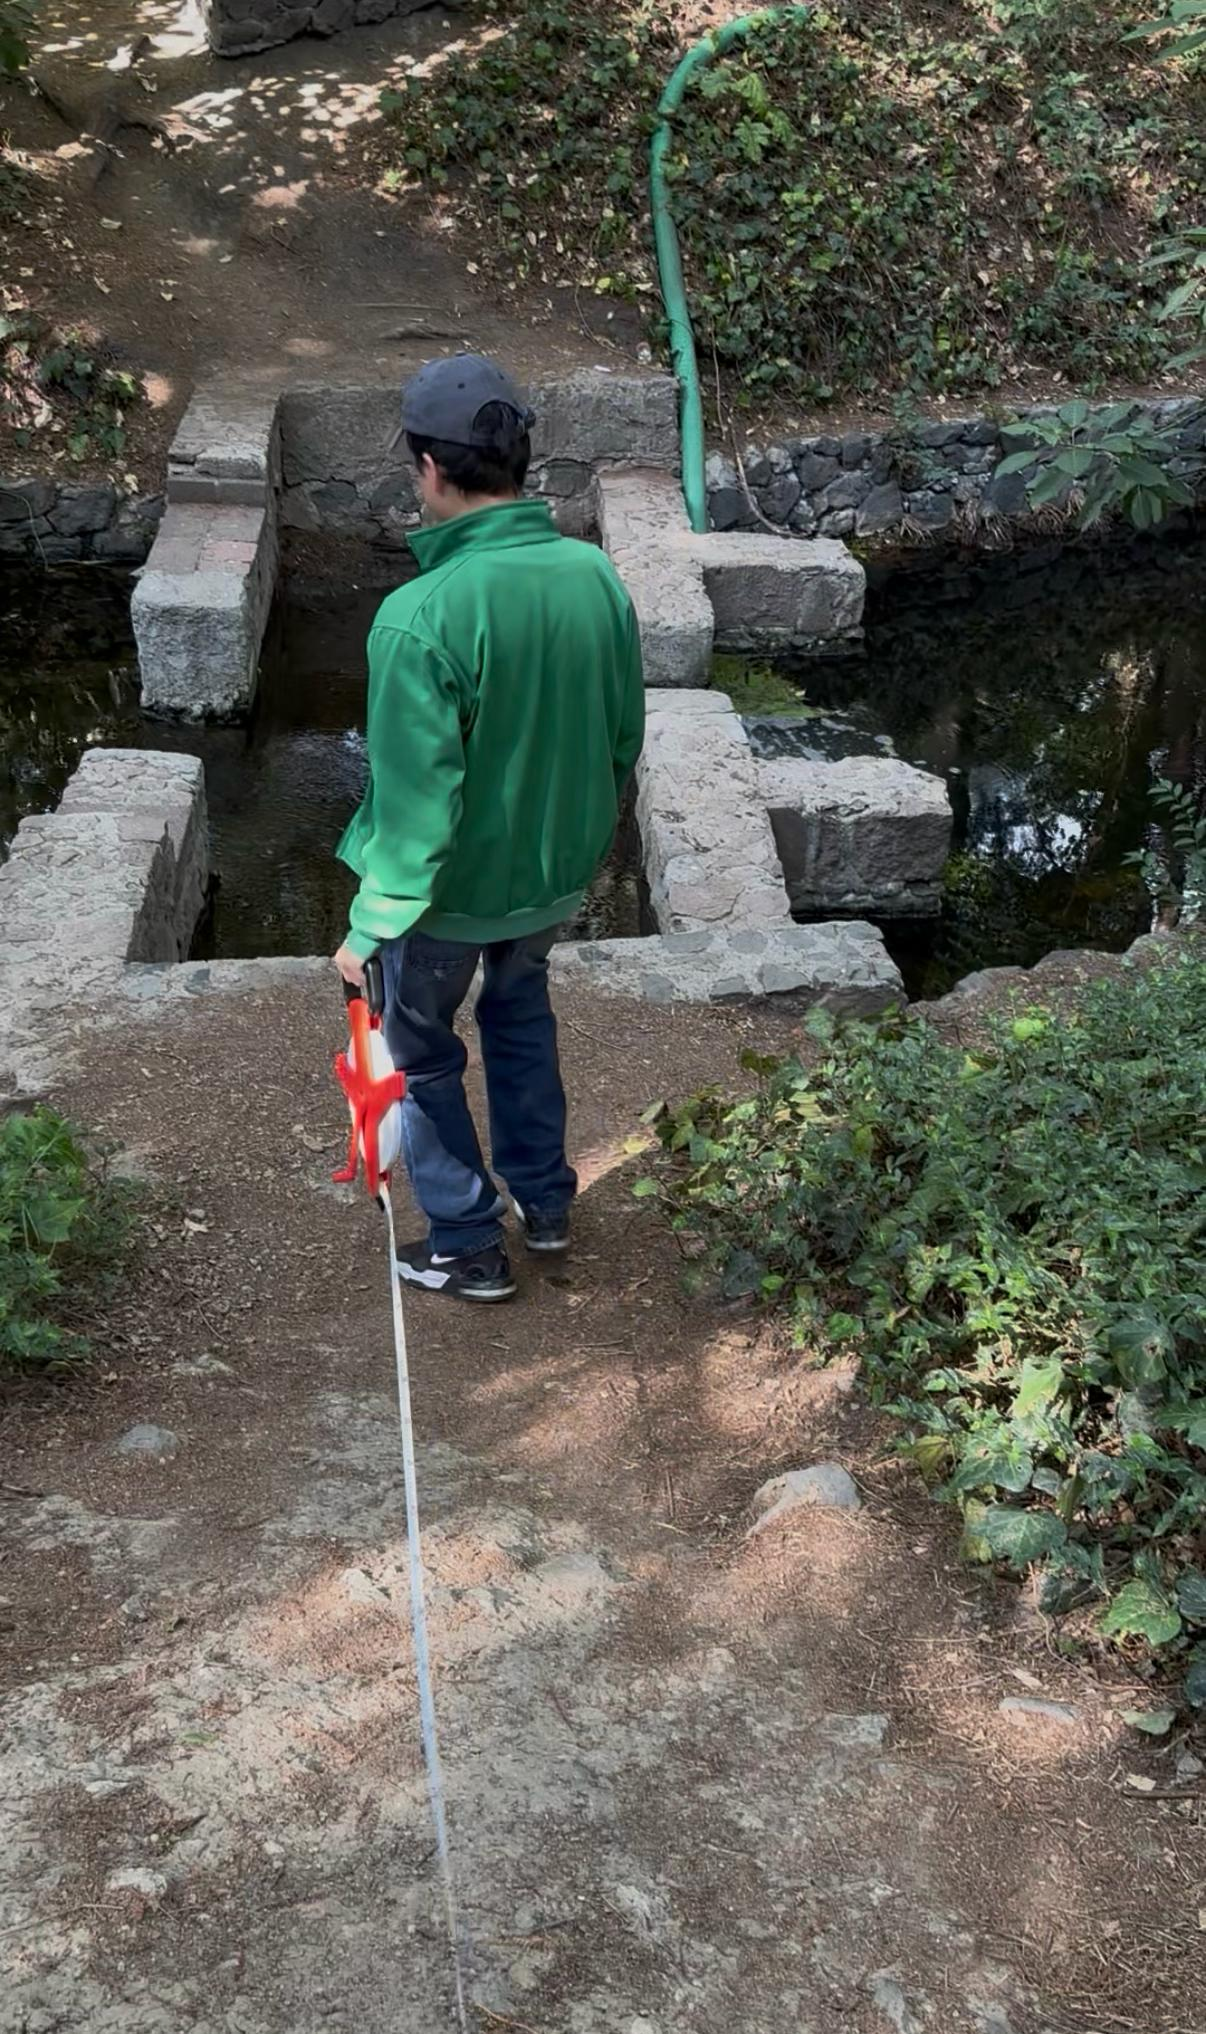
\includegraphics[width=0.6\textwidth]{../../Archivos/Imagenes_Logos/E1.png}
    \caption{Pag58}
    \label{fig:Pag58}
\end{figure}

\begin{figure}[H]
    \centering
    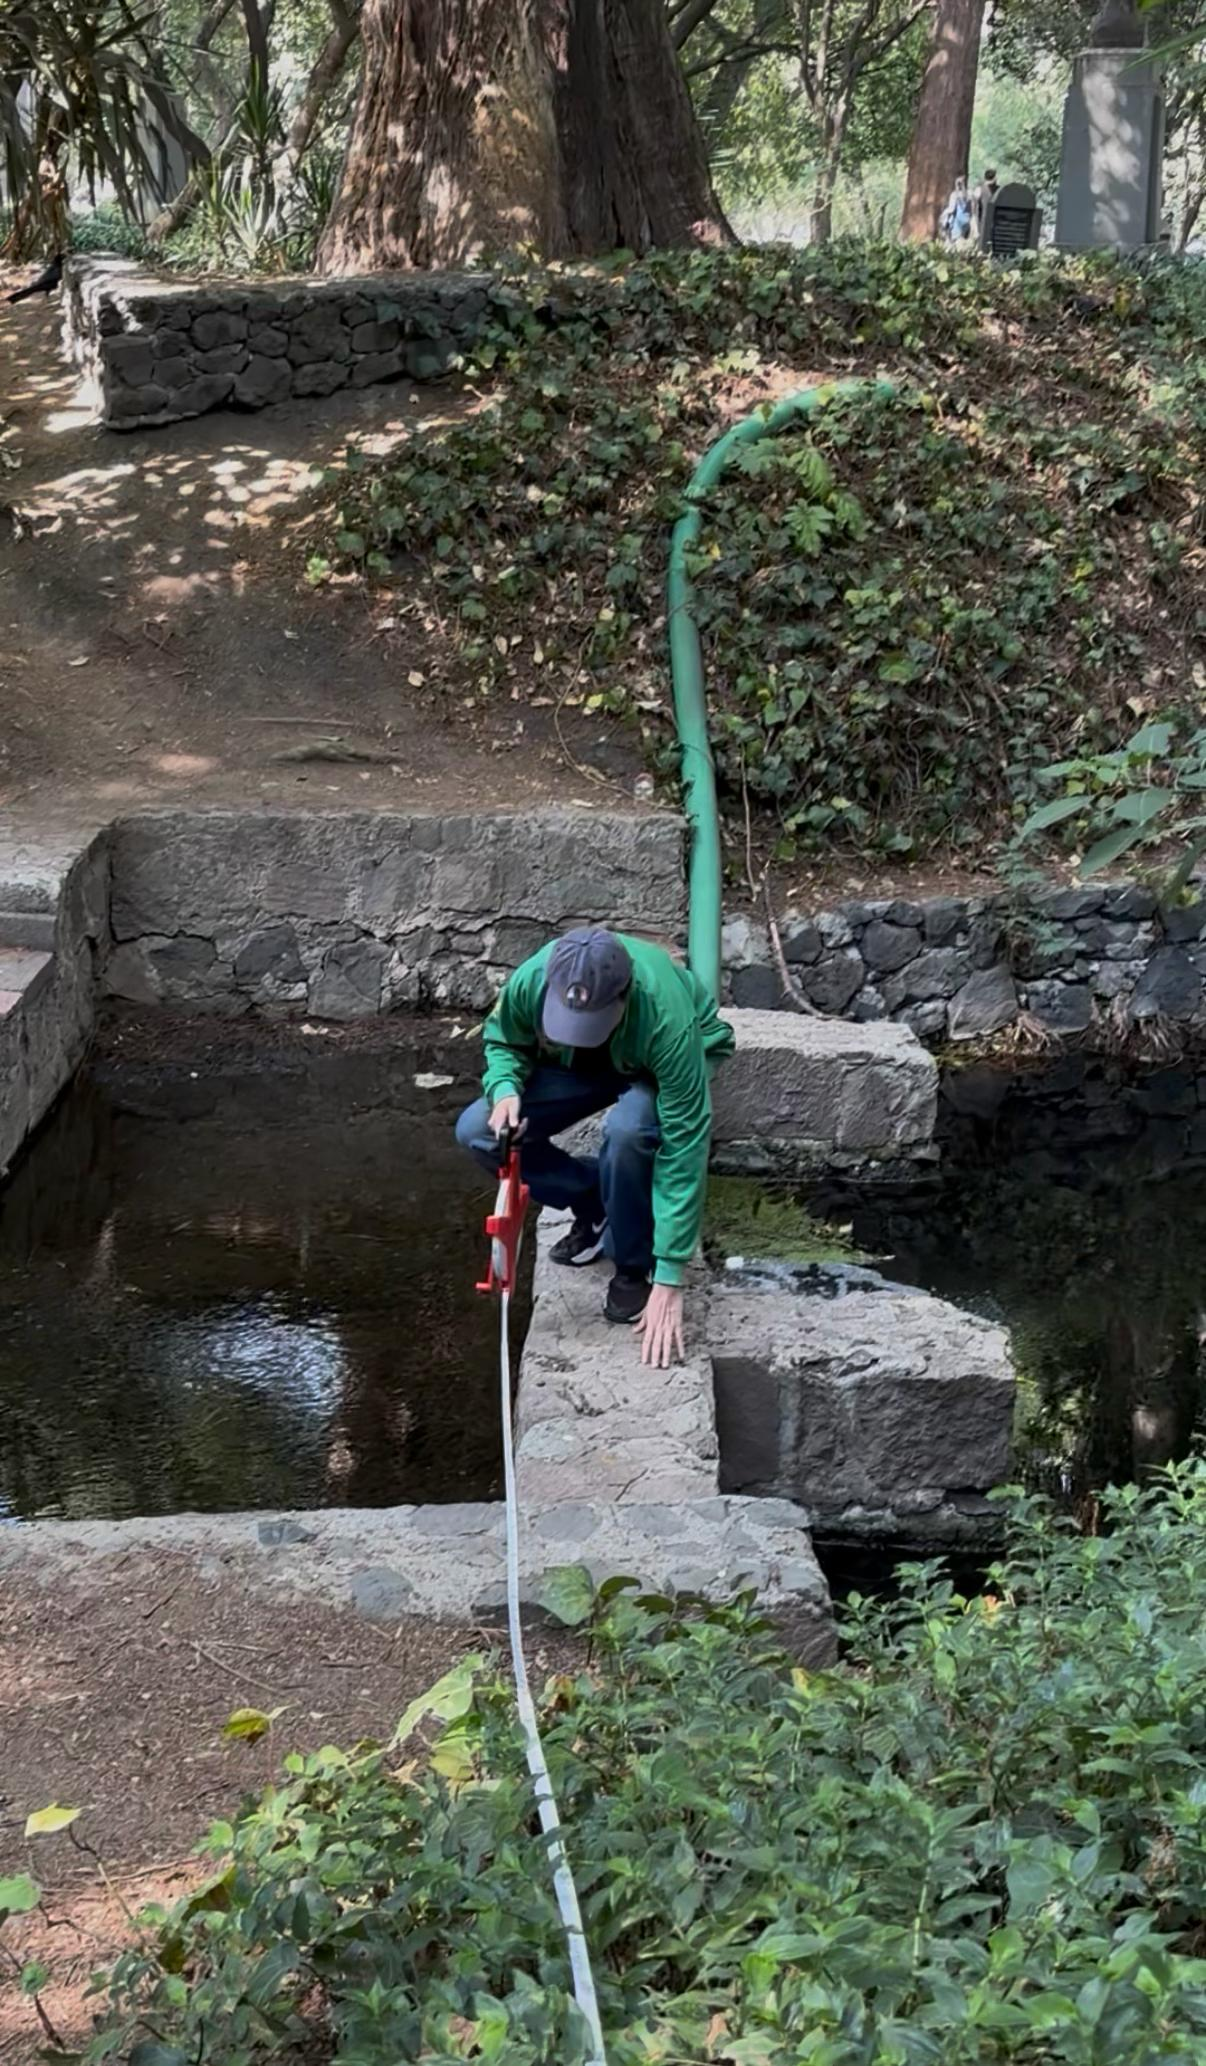
\includegraphics[width=0.6\textwidth]{../../Archivos/Imagenes_Logos/E2.png}
    \caption{Pag59}
    \label{fig:Pag59}
\end{figure}

\begin{figure}[H]
    \centering
    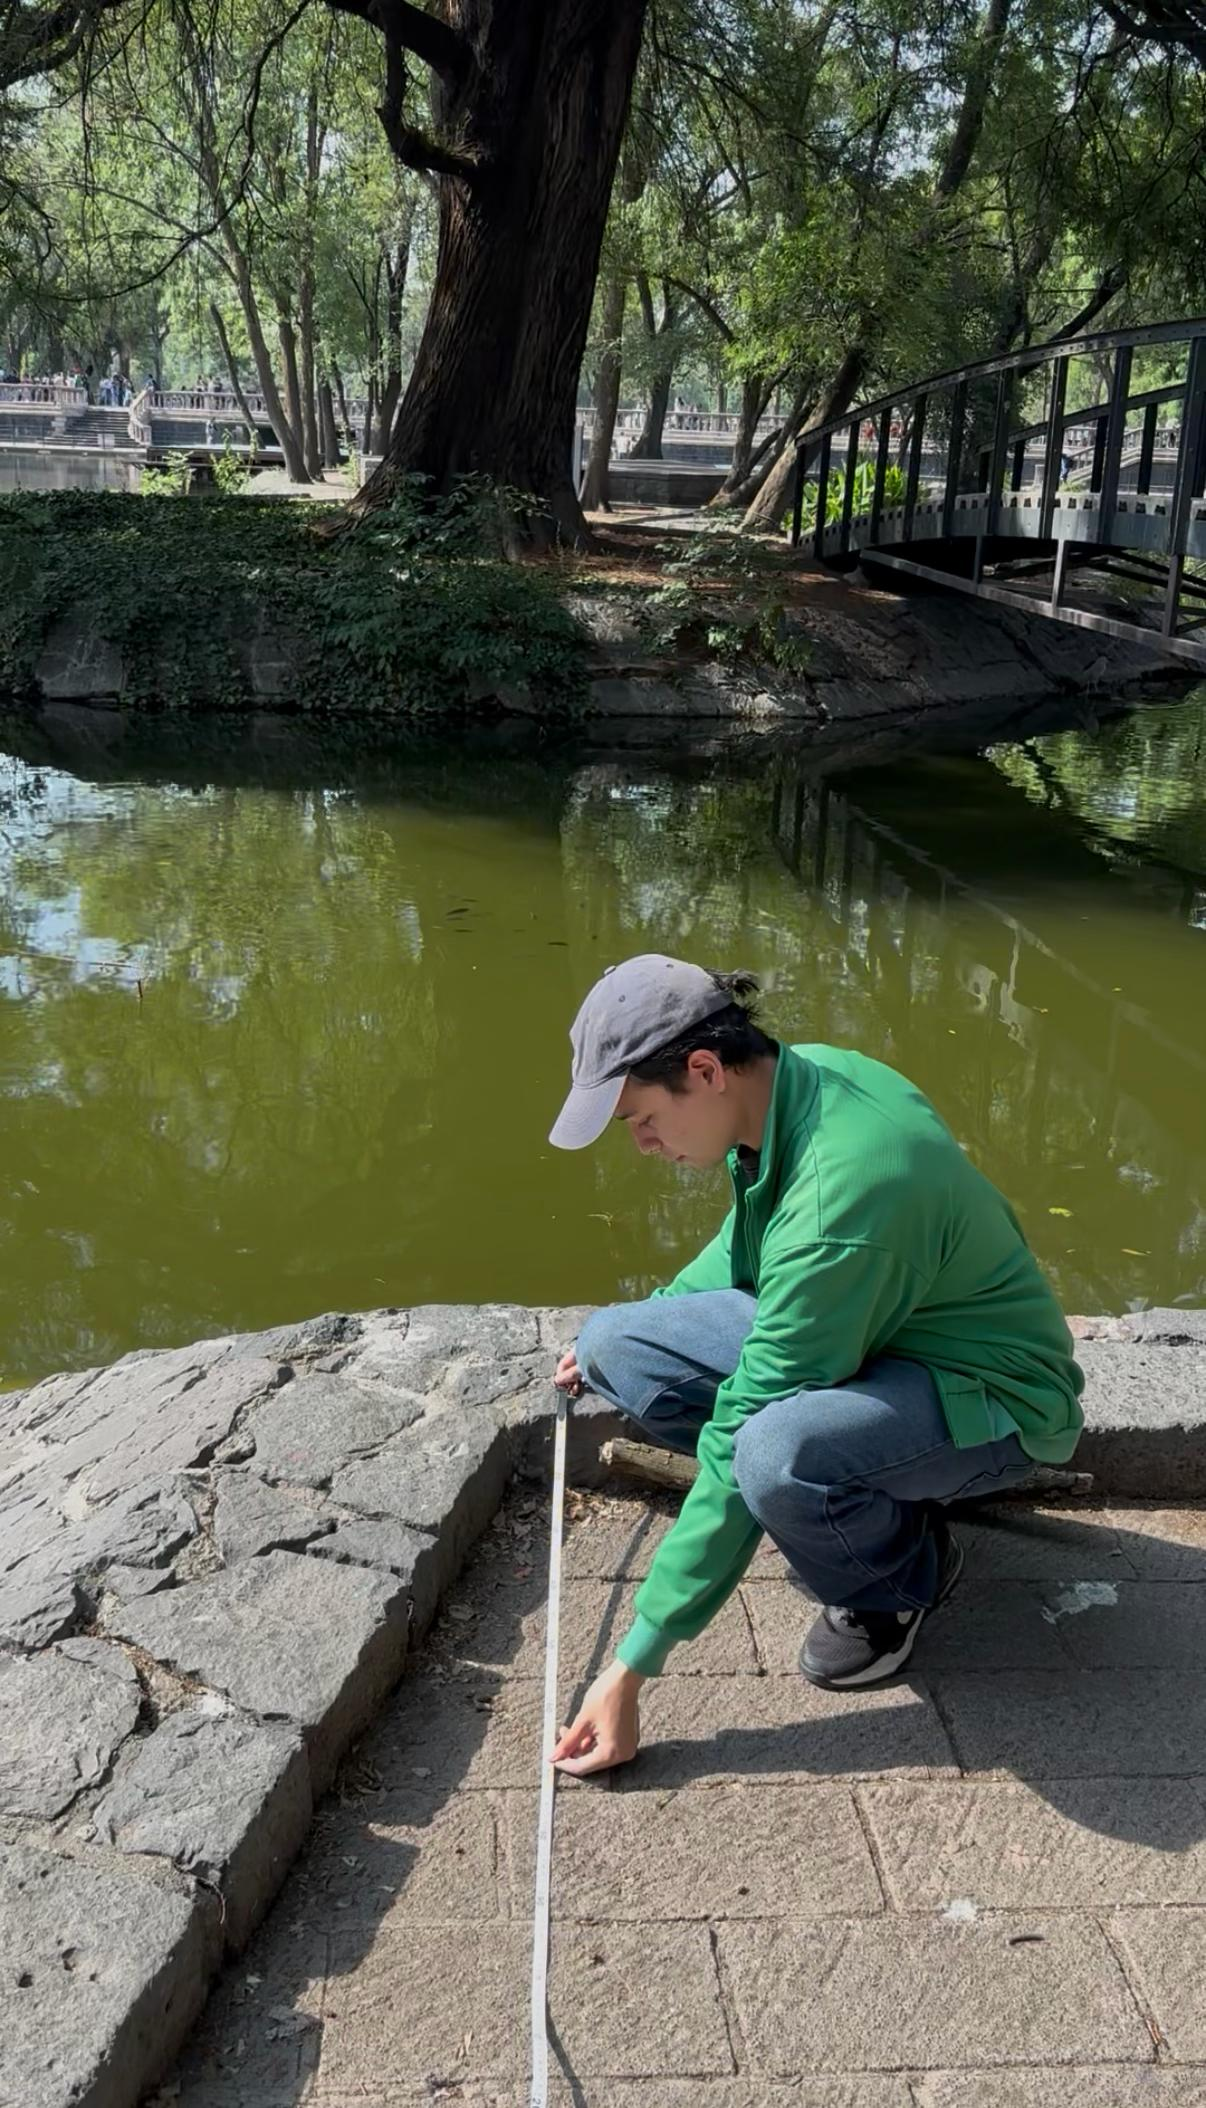
\includegraphics[width=0.6\textwidth]{../../Archivos/Imagenes_Logos/E3.png}
    \caption{Pag60}
    \label{fig:Pag60}
\end{figure}

\end{document}